\section{SilverTorch Model Design}
\label{sec:4}
The idea of SilverTorch is to define the recommendation serving components as model, which provides a unified interface and enables the co-design between components. This section first introduces key abstractions in SilverTorch, and discuss in-model design containing the bloom index based feature filtering and a fused Int8 ANN search. Finally, we discuss a co-designed ANN search and feature filtering algorithm.

\underline{Index as Model}. Both ANN search and feature filtering are required to efficiently serve online retrieval requests within a latency budget. A recommendation query can be defined as follows:
\begin{verbatim}
ANN_Index(user_emb) AND 
(feature1=value1 OR feature1=value2 OR ...) AND
(feature3=value3 OR feature4=value4 OR ...) AND..
\end{verbatim}
A concrete example is below:
\begin{verbatim}
ANN_Index(user_emb) AND item_country = "US"
AND (item_lang = "EN" OR item_lang = "ES")
\end{verbatim}
\noindent The user embedding (user\_emb) is computed from User Tower, while item attributes such as item\_country and item\_lang are defined during publish. Query parameters include user-specific features (user\_emb, user\_country, user\_lang1, user\_lang2). 
To support the ANN search sub-query, SilverTorch provides a fused Int8 ANN kernel leveraging the IVF(inverted file indexing) algorithm. It first probes a subset of clusters close to the query. Then it calculates topk items within each cluster and generates the global topk result.
For feature filtering, we propose bloom index, which leverage efficient bit-wise computation on GPUs. We optimize the feature filtering with ANN search by proposing a co-designed index.
During online serving, the retrieval model is executed in a simplified predictor, which eliminates the communication between standalone indexing services and fully utilizes GPU resources.

\underline{Embedding and Feature Cache}. For the OverArch, to reduce online inference cost, SilverTorch pre-computes item embeddings during publish and populates results on GPUs as embedding cache. The in-model cache look-up removes the dependency of caching services and keeps the computation inside the GPUs. Similarly, the static features are cached on GPUs.

\subsection{Bloom Index}
\label{sec:4.1}
A recommendation query contains feature filtering to match item features with user attributes, represented as nested logical expressions. A common approach is inverted index, which maps each feature value to a posting list of matching items.
However, inverted index is not well suited to GPUs. First, unlike text terms in web search that follow a Zipf distribution with many short postings, recommendation features are typically broad and dense. The lack of sparsity eliminates the efficiency gains that inverted indexes provide in needle-in-the-haystack scenarios. Second, the list-based structure of inverted indexes is inherently sequential and misaligned with GPU parallelism. These limitations motivate our design of a more efficient feature filtering index for recommendation.

We revisit feature filtering problem with two key observations. 
First, the query structure is known in advance, enabling optimized data layouts.
Second, recommendation items contain few feature values per item compared to high-cardinality text search.
Forward index offers stateless query evaluation, enabling parallel processing across all items—a natural fit for GPUs.
Each thread evaluates a partition of items and matches local results, improving efficiency in high-recall scenarios compared to inverted index's multi-way merge. We can represent forward index with three tensors: feature\_ids for identifiers, feature\_values tensor for grouped values per (item, feature) pair, and feature\_offsets tensor for indexing feature\_values, defining value boundaries for each feature. The
feature\_values for a given (item, feature\_id) pair are sorted.
%During filtering, different thread processes a partition of items and matches local results. This approach could largely improve efficiency in high-recall search scenario compared to the multi-way merge of inverted index. In SilverTorch, we define the operators in PyTorch, therefore, the tensor layout of forward index can be represented as following tensors: feature\_ids tensor for feature identifiers, feature\_values tensor for grouped feature values by (item, feature\_ids), and feature\_offsets tensor to index feature\_values, defining value boundaries for each feature. The feature\_values for a given (item, feature\_id) pair are sorted. 
Despite enabling parallelism, forward index has limitations. Offset lookups for each (item, feature) pair create irregular and non-contiguous memory access patterns, limiting throughput when multiple filter conditions are matched. Since the GPU memory is expensive and largely impact the system throughput, forward index requires a large memory footprint because it stores the feature values using int64. To address these limitations, we propose the Bloom Index, a bloom-filter-based GPU indexing structure. It addresses the warp divergence of forward index, ensures contiguous memory access through bitwise operations, and significantly reduces memory consumption by representing each item with compact signature bits.


\begin{figure*}[h]
    \centering
    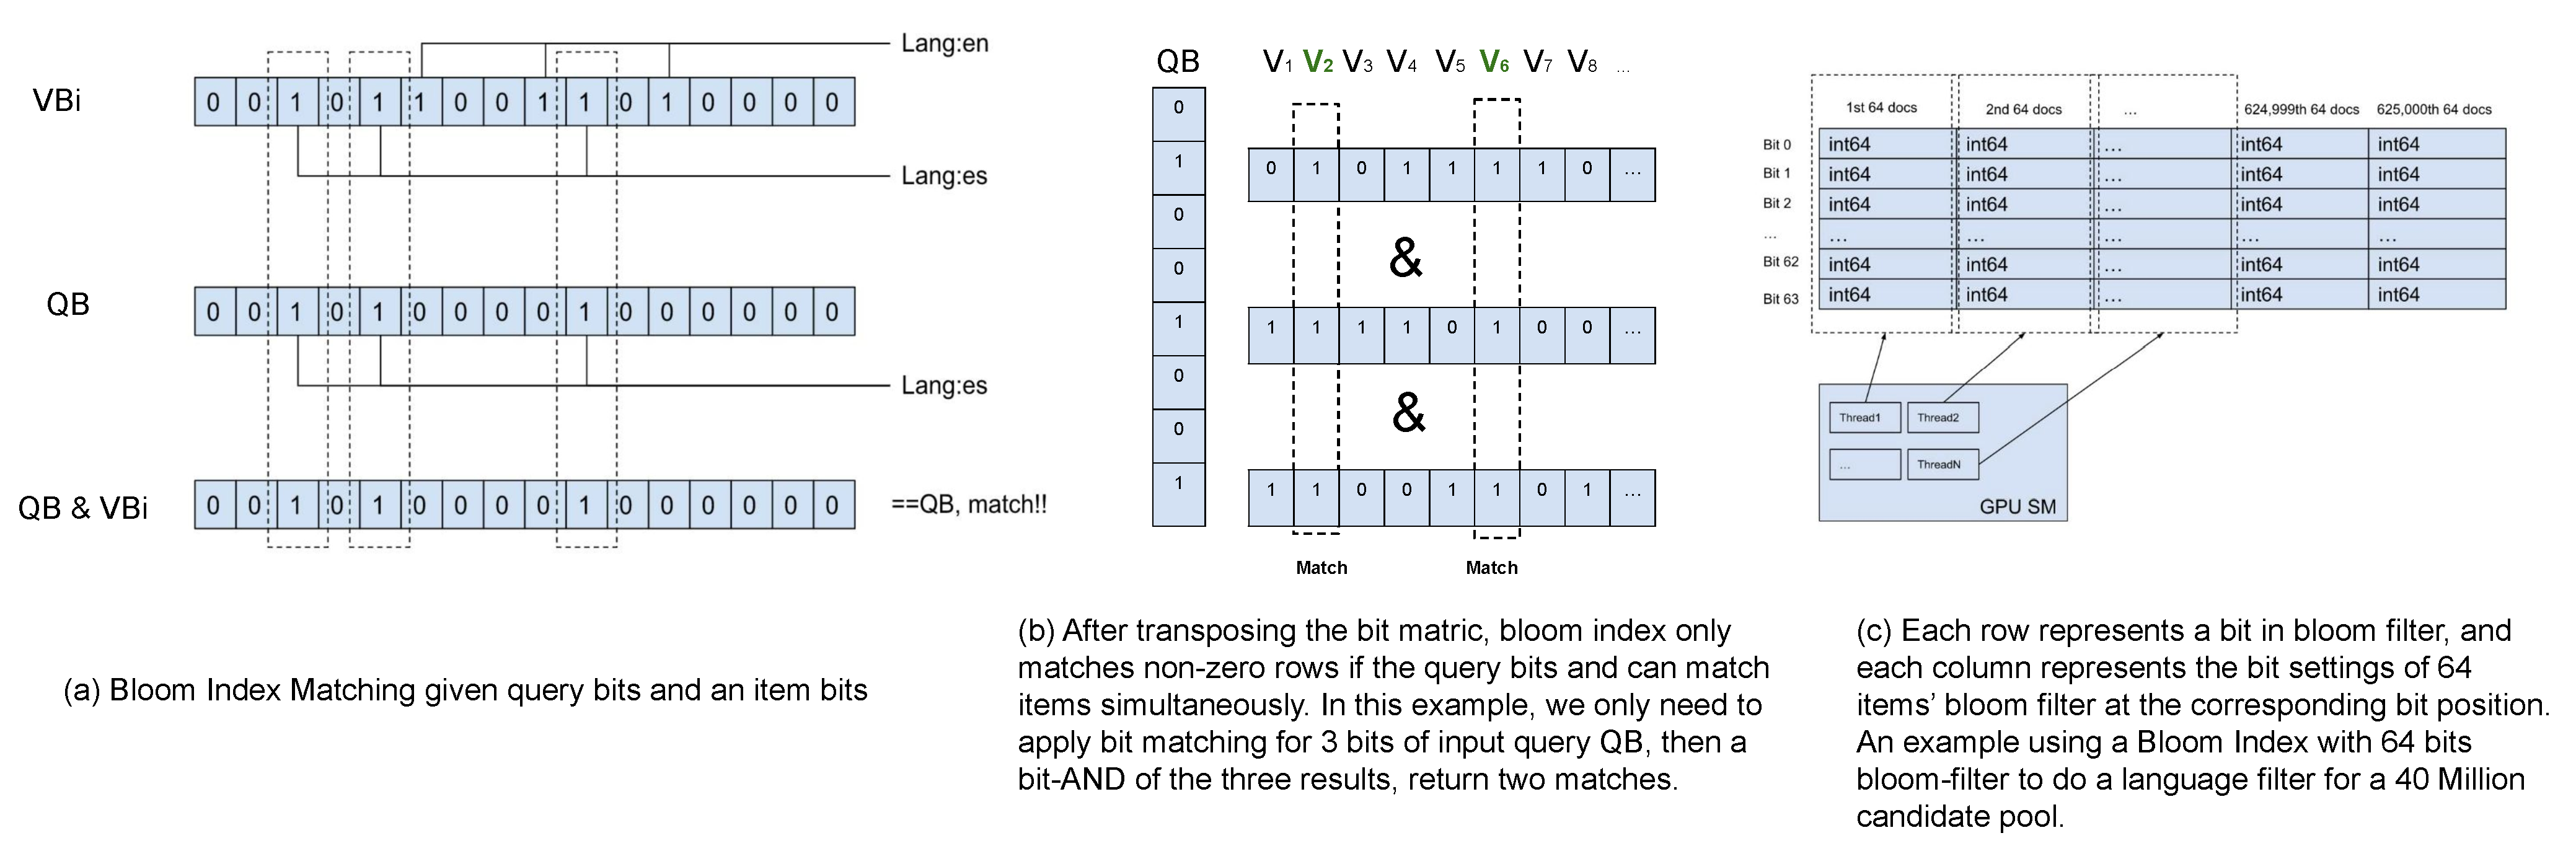
\includegraphics[width=1.0\textwidth]
    {figures/system-design/bloom_all.pdf}
        \caption{Explanations of Bloom Index Algorithm for Feature Filtering}
    \label{fig:bloom_all}
\end{figure*}

We formulate the feature filtering problem as follows, given a list of items V, where each item is represented as a list of features:
\begin{equation}
    V = \{ V_i = [f_1, f_2, ... f_t] \}
\end{equation}
Given a query Q, which can also be represented as a list of features:
\begin{equation}
    Q = [f_1, f_2, ... f_t]
\end{equation}
The goal is to find a list of items that meet following criteria:
\begin{equation}
    R = \{ V_i \in V \mid Q \cap V_i == Q \}
\end{equation}
Bloom filter is a hash-based structure used to check whether an element exists in a set. In bloom index design, we construct a M-bit bloom filter for each item, denoted as VB\_i. For each feature, we apply K hash functions to compute hash\_i(feature) \% N and set the corresponding bits in bloom filter to 1. Similarly, we generate a M-bit bloom filter for the filtering query, denoted as QB, and apply previous k hash functions to mark corresponding bits to 1. By applying this to (3), we obtain:
\begin{equation}
    R = \{ V_i \in V,  V_i = VB_i \mid QB  \&  VB_i == QB \}
\end{equation}

To implement (4), each thread iterates through the bits of QB and then iterates each item in its partition to compute the matches. Figure \ref{fig:bloom_all}(a) illustrates this process using a real example. While transforming filtering into bit manipulation of matrix, it has two drawbacks. First, each GPU thread processes one item at a time. Second, items corresponding to 0 bits in QB are also evaluated. We optimize it by only examining the bits set to 1 in QB. If all the corresponding bits in VB\_i are also 1, it is a match. By rotating the matrix, we isolate the rows containing 1 bits in the query and skip the rest. Such transpose allowing multiple items to be matched simultaneously while eliminating the bit masks necessary to perform Boolean computation.
We only calculate rows containing the 1 bit from QB by performing a bit-wise AND operation between all the matched rows. Any 0 bits indicate a non-match, while 1 bits indicate a match. Figure \ref{fig:bloom_all}(b) shows the process how our bloom index works. QB is a 8-bit bloom filter, and V2 and V6 are matches.
We use a single instruction to execute a 64-bit AND operation (PTX: and.b64), meaning each thread processes 64 items with a single instruction. Comparing to forward index, which matches item-by-item iterative inside a partition and requires a Boolean to store the result for each item, bloom index process 64 items simultaneously and stores the results of 64 items using one Int64. For a case of 40 million items, the data can be splitted into 625,000 partitions. Each thread processes $\frac{625,000}{\text{\#Threads}}$ partitions.
Bloom index leverages bloom filter, which may introduce false positives due to hash collision. By tuning the bloom filter size M and the number of hash functions K based on the number of features N, we could keep the rate very low. Additionally, rare false positive items generated by bloom index in retrieval can always be eliminated by subsequent ranking stages.

\subsection{Fused Int8 ANN Search}
Existing ANN systems such as Faiss and Milvus are general-purpose libraries requiring customization for recommendation use cases. Although both support GPU execution, they impose hard limitations on top-k size. Modern retrieval models use ANN search as a pre-filter returning O(10,000) items, followed by an OverArch model for re-ranking. Consequently, most production systems still rely on CPU-based ANN search due to its scalability and maturity.
To overcome these limitations, we propose a Int8 ANN search kernel in SilverTorch using tensors as index containers. This tensor-native design integrates directly into arbitrary ML serving stack and is inherently parallel-friendly on GPUs. We adopt the clustering-based IVF algorithm with three steps: (1) compute dot products between query and centroid embeddings, (2) search top item embeddings within selected clusters, and (3) identify global top-k across clusters.
We identified the bottleneck in the index selection step, which generates a large temporary tensor to retrieve embeddings for top-k computation. To address this, we introduce a fused index-matmul operator that streams item embeddings directly from the embedding table and computes dot products with batched queries on-the-fly, avoiding intermediate tensor construction. By assigning each warp to process a contiguous tile of items, this operator fully exploits GPU parallelism with coalesced memory access.
We further observe that even precise nearest neighbor results may not yield perfect retrieval accuracy, as dot-product similarity oversimplifies the retrieval model. Additionally, storing complete embedding tensors on GPU becomes a memory bottleneck as candidate pools grow. Based on these observations, we propose Int8 quantized fused ANN search. By representing embeddings with 8-bit integers and leveraging GPU's dp4a instruction (computing four multiply-adds in one instruction), we achieve higher throughput and halve the memory footprint. Quantization occurs during model publish: we compute global min/max values across all embeddings, scale them to [-128, 127], and assign integer representations accordingly.
Our Int8 quantized ANN search shows limited quality loss while significantly improving serving performance. It frees headroom for the OverArch layers to rank more items and improves the end-to-end retrieval accuracy. The algorithm supports large top-k and probe counts; in practice, we observe no recall loss with 64 probes and top-2048.
%Existing ANN systems such as Faiss and Milvus are general-purpose libraries that needs customization for recommendation use. Although both of them support executing ANN search on GPUs, a hard limitation is that both limit the topk. Modern retrieval models adopts ANN search as a pre-filter, returning O(10,000) items, followed by a OverArch to re-rank. Therefore, most of existing systems still build CPU-based ANN search due to its scalability and maturity.
%To overcome the limitation, we propose a Int8 ANN search kernel in SilverTorch, leveraging tensor as the index container. The tensor-native design can be directly incorporated into any ML model serving stack and is by nature parallel-friendly on GPUs. We adopt the clustering-based IVF algorithm that follows three steps. First, it calculates the dot product between query embedding and the centroid embeddings. Second, it searches the top item embeddings inside selected clusters. Third, it identifies the global topk across the clusters.
%We found the bottleneck of this algorithm lies in the index selection step that generates a temporary embedding indices tensor to retrieve embeddings for compute the topk. Additionally, the performance of index selection operator itself is slow. We introduce a fused index-matmul operator after probing, it streams item embeddings directly from the embedding table and computes dot-product with batched queries on-the-fly, avoiding the construction of a large intermediate tensor. By assigning each warp to process a contiguous tile of items, this operator fully exploits GPU parallelism and achieves coalesced memory access.

%In recommendation systems, we found that even if we could get precise nearest neighbor search results, overall accuracy for retrieval may not be perfect. The reason is the dot-product over simplifies the retrieval model. Additionally, since the ANN index stores complete embedding tensors on GPU, it becomes the bottleneck as candidate pool grows. Base on these observations, we propose a INT8 quantized fused ANN search algorithm. By representing each embedding with 8-bit integer and leveraging GPU instructions such as dp4a(an instruction that capable of computing four multiplications and additions in a single instruction), we achieve much higher throughput and lower memory footprint by half. The quantization process occurs during SilverTorch model publish, involving computing the global min and max values among all the embedding values. Then the max and min values are scaled to fit within the range [-128, 127], representing the range that can be represented by each integer. Each embedding is then assigned an integer representation based on the range it falls into, using the corresponding integer within [-128, 127]. We found that our INT8 quantized fused ANN search has limited quality loss but can improve the serving performance a lot. The performance headroom can fund serving more deep OverArch layers for ranking more items in retrieval. Our algorithm could effectively support searching arbitrary topk and number of probes. In practice, it could achieve searching with 64 probes of top 2048 items without any recall loss.

\subsection{ANN and Filtering Co-design}
\label{sec:4.3}
SilverTorch unifies ANN search and feature filtering operators within the PyTorch stack, with all indexes stored as GPU tensors in the same runtime. This unified design provides opportunities to co-design these operators. We observe that although full bloom filtering is accurate, much of the computation is wasted—items passing the filter are often excluded by ANN probing, which only scores items within selected clusters. This insight motivates our co-designed approach that reverses the traditional order of operations: we first identify which clusters to probe, then apply filtering only to items within those clusters. The results remain the same. Our implementation leverages several GPU-friendly optimizations. The ANN search operator accepts a bit mask from the bloom index using 1-bit per item instead of PyTorch's native 8-bit boolean, conserving memory and reducing global memory bandwidth. For complex filter queries containing multiple logical expressions (AND, OR, NOT), we parse queries and pre-compute each feature's bloom result, storing operators and results in an operation array. During evaluation, we process this array sequentially using a stack to push temporary results and pop for logical computation. Since a single batch may contain hundreds of sub-queries requiring extensive bloom computation, and GPU memory bounds model throughput, reducing the filtering scope becomes critical.

Algorithm~\ref{alg:partial_bloom} presents our co-designed index. In Phase 1, we compute query-centroid distances and select the top-$n_p$ clusters, identifying which items will actually be scored. In Phase 2, we compute bloom filter results only for items within selected clusters, generating compact bit masks $\mathbf{M}_c$ for each cluster. Phase 3 computes embedding similarity scores only for items passing the partial bloom filter, combining filtering and scoring in a single GPU kernel pass. Finally, Phase 4 aggregates scores across all probed clusters and returns the top-$k$ item IDs and scores. For an index with 81 million items across 9,000 clusters, using 256 probes processes only 2.3 million items (2.8), achieving a 30$\times$ reduction in both filtering computation and GPU scratch memory.

%In service-based model serving systems, data are transferred between ANN search, feature filtering and remaining model inference components. There are services that provide a interface to support both ANN search and feature filtering(e.g., Elasticsearch or MongoDB), but data are stored with different formats for filtering and ANN search. In contrast, SilverTorch unifies the serving operators within PyTorch stack. All operators are running in the same runtime environment and different types of indexes are stored as tensors in GPU memory. This provides us the opportunities to jointly optimize the operators. In our Int8 ANN search operator, we support passing a bit mask output from bloom index. While PyTorch native supports Boolean as mask(8 bits per item), we use a bit mask with one bit for each item. It can both conserves memory and enhances performance by reducing the amount of data that need to be loaded from GPU's global memory. Taking the bit mask, before executing the final step of calculating topk results, the ANN search operator applies the bloom bitmask to filter out unmatched items and then apply topk calculation. Such flexibility and co-design benefit from SilverTorch's model-based index design.
%In real use cases, a feature filtering query can be very complex that containing multiple logical expression of different matches. To support this, we parse the query and pre-compute each feature's bloom result. We store each operator(e.g, And, OR, NOT) followed by the bloom result in an operation array. During serving, we go through this operation array sequentially, leveraging a stack to push temporary computation results and pop for logical computation between bloom results. A single batch queries could contain hundreds of sub-queries for feature filtering in total, thus having hundreds of bloom search computation. Additionally, the throughput of SilverTorch models was bounded by GPU memory. To solve these challenges, we propose feature filtering and ANN search by proposing a partial ANN search algorithm with bloom results, named as ANN and filtering co-designed index.
%The co-designed index leverages the fact that only items within selected clusters need to apply the feature filtering. By calculating bloom results for the items in selected clusters only, we can return equivalent results while significantly reducing both computation and memory utilization for each request. For a case of 81 million items with 9000 clusters, each cluster has 9000 items on average. Bloom index is applied to only 2.3 million items(2.8\% of the full items with 256 probes, achieving $30\times$ saving of feature filtering compute and reduce $30\times$ of scratch memory during serving.

\begin{algorithm}[t]
\caption{Co-designed ANN Search with Partial Bloom Filtering}
\label{alg:partial_bloom}
\begin{algorithmic}[1]
\Require Query embedding $\mathbf{q}$, filter predicates $\mathcal{F}$, item embeddings $\mathbf{E}$, cluster centroids $\mathbf{C}$, cluster offsets $\mathbf{O}$, cluster lengths $\mathbf{L}$, Bloom index $\mathbf{B}$, number of probes $n_p$, $k$
\Ensure Top-$k$ item IDs and scores
\State \textbf{// Phase 1: ANN Probing}
\State $\mathbf{D} \gets \mathrm{Distance}(\mathbf{q}, \mathbf{C})$
\State $\mathcal{P} \gets \mathrm{TopK}(\mathbf{D}, n_p)$
\State \textbf{// Phase 2: Partial Filtering on selected probes}
\State \textbf{for all} cluster $c \in \mathcal{P}$:
\State \quad $s_c \gets \mathbf{O}[c]$, $l_c \gets \mathbf{L}[c]$
\State \quad $\mathbf{M}_c \gets \mathrm{BloomSearch}(\mathbf{B}, \mathcal{F}, s_c, l_c)$
\State \textbf{// Phase 3: Fused Scoring with Partial Masks}
\State $\mathbf{S} \gets \emptyset$, $\mathbf{I} \gets \emptyset$ \Comment{Init scores and indices}
\State \textbf{for all} cluster $c \in \mathcal{P}$, item $d \in c$ where $\mathbf{M}_c[d] = 1$:
\State \quad $\mathbf{S} \gets \mathbf{S} \cup \{\langle \mathbf{q}, \mathbf{E}[d] \rangle\}$, $\mathbf{I} \gets \mathbf{I} \cup \{d\}$
\State \textbf{// Phase 4: Global Top-K}
\State $\mathbf{R} \gets \mathrm{ArgTopK}(\mathbf{S}, k)$
\State $\mathbf{S}^* \gets \mathbf{S}[\mathbf{R}]$, $\mathbf{I}^* \gets \mathbf{I}[\mathbf{R}]$
\State \Return $(\mathbf{I}^*, \mathbf{S}^*)$ \Comment{Item IDs and scores}
\end{algorithmic}
\end{algorithm}